\documentclass[tikz,border=2pt]{standalone}
% Shared Figure architecture visual system for all four main-text figures.
\usepackage[T1]{fontenc}
\usepackage{charter}
\usepackage[scaled=0.90]{helvet}
\usepackage{amsmath,amssymb}
\renewcommand{\Pr}{\mathbb{P}}
\usepackage{xcolor}
\usepackage{tikz}
\usepackage{pgfplots}
\pgfplotsset{compat=1.18}
\usetikzlibrary{arrows.meta,calc,positioning,fit,decorations.pathreplacing,shapes.geometric,backgrounds}
\definecolor{figNavy}{RGB}{0,63,92}
\definecolor{figBlue}{RGB}{0,101,165}
\definecolor{figSky}{RGB}{226,241,249}
\definecolor{figTeal}{RGB}{0,125,112}
\definecolor{figMint}{RGB}{224,243,239}
\definecolor{figOrange}{RGB}{222,102,35}
\definecolor{figPeach}{RGB}{252,235,224}
\definecolor{figRed}{RGB}{145,43,55}
\definecolor{figInk}{RGB}{35,45,51}
\definecolor{figGray}{RGB}{103,115,123}
\definecolor{figRule}{RGB}{194,202,208}
\definecolor{figPale}{RGB}{248,250,251}
\definecolor{figWhite}{RGB}{255,255,255}
\tikzset{
  figpanel/.style={draw=figRule,line width=0.55pt,rounded corners=2.4pt,fill=figWhite},
  figtag/.style={circle,fill=figBlue,text=figWhite,minimum size=4.3mm,inner sep=0pt,font=\sffamily\bfseries\fontsize{7.5}{8}\selectfont},
  figtitle/.style={font=\sffamily\bfseries\fontsize{8.5}{10}\selectfont,text=figNavy,anchor=west},
  figsubtitle/.style={font=\sffamily\fontsize{6.8}{8}\selectfont,text=figGray,align=left},
  figbody/.style={font=\sffamily\fontsize{7}{8.4}\selectfont,text=figInk,align=center},
  figsmall/.style={font=\sffamily\fontsize{6.2}{7.4}\selectfont,text=figGray,align=center},
  figmath/.style={font=\fontsize{7.4}{8.8}\selectfont,text=figInk,align=center},
  figflow/.style={-{Stealth[length=2.0mm,width=1.4mm]},draw=figBlue,line width=0.85pt},
  figflowgray/.style={-{Stealth[length=1.8mm,width=1.25mm]},draw=figGray,line width=0.75pt},
  figfloworange/.style={-{Stealth[length=2.0mm,width=1.4mm]},draw=figOrange,line width=0.85pt},
  figbluebox/.style={draw=figBlue,line width=0.65pt,fill=figSky,rounded corners=2.2pt},
  figorangebox/.style={draw=figOrange,line width=0.65pt,fill=figPeach,rounded corners=2.2pt},
  figtealbox/.style={draw=figTeal,line width=0.65pt,fill=figMint,rounded corners=2.2pt},
  figgraybox/.style={draw=figRule,line width=0.6pt,fill=figPale,rounded corners=2.2pt},
}
\newcommand{\PanelHeading}[4]{%
  \node[figtag] at (#1,#2) {#3};%
  \node[figtitle] at ({#1+0.32},#2) {#4};%
}

\begin{document}
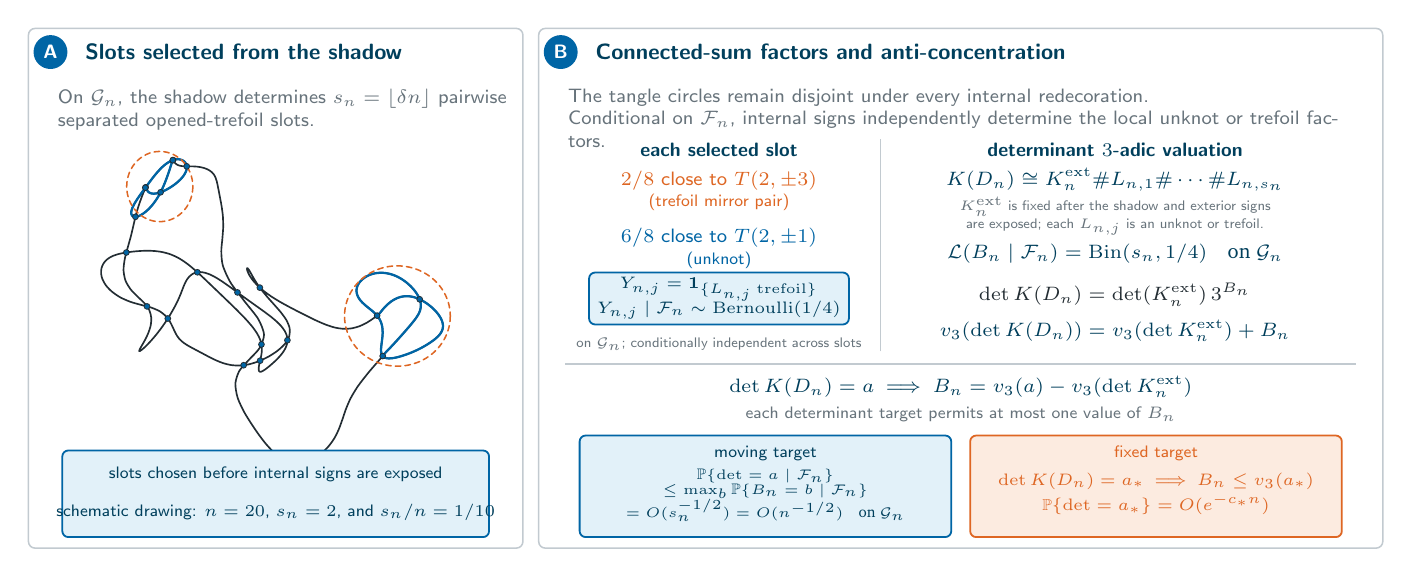
\begin{tikzpicture}[x=1cm,y=1cm]
% Two-panel mechanism figure: concrete shadow and the merged local-to-global argument.
\draw[figpanel] (0,0) rectangle (6.28,6.60);
\draw[figpanel] (6.48,0) rectangle (17.20,6.60);

% A. Concrete shadow-first selection.
\PanelHeading{0.28}{6.30}{A}{Slots selected from the shadow}
\node[figsubtitle,anchor=north west,text width=5.70cm] at (0.25,5.95) {On $\mathcal G_n$, the shadow determines $s_n=\lfloor\delta n\rfloor$ pairwise separated opened-trefoil slots.};
\begin{scope}[every plot/.append style={smooth,tension=0.45}]
% Close the imported one-component SVG path explicitly; its sampled endpoints
% otherwise leave a tiny white break in the lower strand.
\draw[draw=figInk,line width=0.60pt,line cap=round,line join=round]
  (3.2237,1.1400) .. controls (3.2100,1.1460) and (3.1945,1.1565) .. (3.1813,1.1668);
\draw[draw=figInk,line width=0.60pt,line cap=round,line join=round] plot coordinates {(3.1813,1.1668) (3.0966,1.2365) (3.0124,1.3279) (2.9262,1.4404) (2.8342,1.5747) (2.7377,1.7319) (2.6567,1.9095) (2.6282,2.0903) (2.6781,2.2506) (2.7986,2.3898) (2.9337,2.5383) (2.9922,2.7123) (2.9180,2.9105) (2.7424,3.1370) (2.5646,3.3760) (2.4684,3.5899) (2.4495,3.7682) (2.4625,3.9252) (2.4734,4.0734) (2.4696,4.2137) (2.4536,4.3403) (2.4339,4.4480) (2.4170,4.5357) (2.4034,4.6058) (2.3910,4.6613) (2.3763,4.7058) (2.3572,4.7419) (2.3326,4.7712) (2.3025,4.7948) (2.2675,4.8136) (2.2288,4.8279) (2.1877,4.8379) (2.1456,4.8443) (2.1034,4.8474) (2.0621,4.8485) (2.0228,4.8485) (1.9857,4.8491) (1.9513,4.8514) (1.9203,4.8570) (1.8929,4.8671) (1.8695,4.8824) (1.8504,4.9036) (1.8355,4.9304) (1.8207,4.8974) (1.8123,4.8682) (1.8028,4.8375) (1.7925,4.8057) (1.7815,4.7729) (1.7699,4.7393) (1.7577,4.7053) (1.7449,4.6711) (1.7315,4.6369) (1.7174,4.6030) (1.7025,4.5694) (1.6870,4.5365) (1.6706,4.5044) (1.6532,4.4733) (1.6351,4.4432) (1.6160,4.4142) (1.5963,4.3867) (1.5759,4.3606) (1.5549,4.3361) (1.5336,4.3134) (1.5122,4.2925) (1.4907,4.2737) (1.4695,4.2570) (1.4488,4.2427) (1.4288,4.2307) (1.4096,4.2212) (1.3914,4.2142) (1.3747,4.2097) (1.3592,4.2077) (1.3455,4.2083) (1.3335,4.2114) (1.3236,4.2169) (1.3156,4.2247) (1.3100,4.2348) (1.3066,4.2471) (1.3058,4.2615) (1.3074,4.2779) (1.3116,4.2963) (1.3184,4.3165) (1.3279,4.3386) (1.3400,4.3625) (1.3544,4.3880) (1.3713,4.4152) (1.3901,4.4441) (1.4110,4.4744) (1.4335,4.5063) (1.4572,4.5393) (1.4820,4.5734) (1.5076,4.6083) (1.5339,4.6435) (1.5604,4.6786) (1.5873,4.7132) (1.6143,4.7468) (1.6415,4.7787) (1.6688,4.8085) (1.6960,4.8358) (1.7231,4.8603) (1.7501,4.8816) (1.7766,4.8994) (1.8025,4.9140) (1.8275,4.9248) (1.8517,4.9326) (1.8746,4.9370) (1.8962,4.9384) (1.9162,4.9371) (1.9345,4.9335) (1.9509,4.9277) (1.9655,4.9199) (1.9780,4.9106) (1.9886,4.8999) (1.9970,4.8881) (2.0035,4.8754) (2.0079,4.8619) (2.0104,4.8479) (2.0108,4.8332) (2.0096,4.8184) (2.0065,4.8031) (2.0017,4.7878) (1.9954,4.7722) (1.9874,4.7566) (1.9779,4.7409) (1.9671,4.7252) (1.9548,4.7095) (1.9413,4.6938) (1.9265,4.6783) (1.9103,4.6628) (1.8931,4.6475) (1.8747,4.6324) (1.8554,4.6174) (1.8350,4.6027) (1.8138,4.5884) (1.7919,4.5746) (1.7694,4.5615) (1.7466,4.5491) (1.7234,4.5377) (1.7002,4.5275) (1.6772,4.5187) (1.6545,4.5115) (1.6325,4.5061) (1.6114,4.5028) (1.5914,4.5015) (1.5726,4.5027) (1.5555,4.5063) (1.5403,4.5124) (1.5269,4.5210) (1.5157,4.5321) (1.5067,4.5457) (1.5000,4.5617) (1.4955,4.5801) (1.4595,4.5118) (1.4077,4.3721) (1.3666,4.2375) (1.3351,4.1052) (1.3032,3.9695) (1.2634,3.8255) (1.2240,3.6753) (1.2077,3.5286) (1.2333,3.3956) (1.3002,3.2834) (1.3893,3.1914) (1.4745,3.1091) (1.5347,3.0225) (1.5601,2.9262) (1.5519,2.8243) (1.5199,2.7258) (1.4782,2.6396) (1.4399,2.5721) (1.4141,2.5264) (1.4055,2.5030) (1.4158,2.5020) (1.4446,2.5226) (1.4906,2.5646) (1.5504,2.6267) (1.6188,2.7059) (1.6891,2.7970) (1.7554,2.8930) (1.8136,2.9868) (1.8624,3.0739) (1.9017,3.1532) (1.9325,3.2253) (1.9580,3.2911) (1.9821,3.3509) (2.0092,3.4037) (2.0422,3.4477) (2.0830,3.4808) (2.1316,3.5007) (2.1871,3.5058) (2.2489,3.4955) (2.3159,3.4705) (2.3880,3.4320) (2.4653,3.3827) (2.5476,3.3252) (2.6343,3.2622) (2.7243,3.1966) (2.8161,3.1304) (2.9072,3.0655) (2.9950,3.0024) (3.0767,2.9410) (3.1488,2.8808) (3.2082,2.8212) (3.2522,2.7621) (3.2792,2.7041) (3.2893,2.6479) (3.2839,2.5939) (3.2656,2.5428) (3.2380,2.4949) (3.2041,2.4505) (3.1676,2.4100) (3.1307,2.3736) (3.0954,2.3414) (3.0631,2.3136) (3.0342,2.2902) (3.0091,2.2713) (2.9877,2.2568) (2.9697,2.2466) (2.9551,2.2407) (2.9434,2.2393) (2.9346,2.2423) (2.9284,2.2496) (2.9248,2.2615) (2.9238,2.2777) (2.9255,2.2985) (2.9297,2.3239) (2.9362,2.3540) (2.9446,2.3890) (2.9536,2.4291) (2.9613,2.4747) (2.9647,2.5261) (2.9600,2.5841) (2.9419,2.6497) (2.9048,2.7247) (2.8432,2.8121) (2.7522,2.9162) (2.6298,3.0408) (2.4808,3.1852) (2.3203,3.3390) (2.1677,3.4835) (2.0317,3.6001) (1.9109,3.6817) (1.8013,3.7319) (1.7005,3.7597) (1.6067,3.7728) (1.5182,3.7768) (1.4335,3.7745) (1.3523,3.7683) (1.2751,3.7593) (1.2027,3.7476) (1.1361,3.7324) (1.0763,3.7122) (1.0243,3.6853) (0.9810,3.6501) (0.9478,3.6056) (0.9271,3.5513) (0.9226,3.4876) (0.9396,3.4153) (0.9840,3.3370) (1.0601,3.2575) (1.1669,3.1845) (1.2954,3.1276) (1.4314,3.0887) (1.5594,3.0546) (1.6673,3.0081) (1.7480,2.9430) (1.8029,2.8660) (1.8411,2.7874) (1.8754,2.7160) (1.9175,2.6556) (1.9730,2.6061) (2.0422,2.5626) (2.1214,2.5199) (2.2065,2.4748) (2.2942,2.4283) (2.3836,2.3845) (2.4755,2.3484) (2.5726,2.3251) (2.6776,2.3185) (2.7927,2.3327) (2.9176,2.3702) (3.0462,2.4304) (3.1658,2.5084) (3.2597,2.5972) (3.3126,2.6925) (3.3173,2.7922) (3.2772,2.8938) (3.2058,2.9946) (3.1206,3.0924) (3.0374,3.1856) (2.9662,3.2717) (2.9102,3.3486) (2.8684,3.4146) (2.8376,3.4685) (2.8148,3.5097) (2.7975,3.5380) (2.7850,3.5533) (2.7773,3.5554) (2.7752,3.5445) (2.7804,3.5212) (2.7951,3.4859) (2.8219,3.4399) (2.8636,3.3848) (2.9223,3.3230) (2.9984,3.2576) (3.0906,3.1917) (3.1961,3.1270) (3.3106,3.0640) (3.4302,3.0017) (3.5509,2.9408) (3.6692,2.8837) (3.7831,2.8354) (3.8926,2.8011) (3.9982,2.7853) (4.1007,2.7905) (4.1997,2.8166) (4.2940,2.8610) (4.3822,2.9184) (4.4492,2.9659) (4.4799,3.0067) (4.5123,3.0455) (4.5469,3.0818) (4.5839,3.1149) (4.6236,3.1441) (4.6661,3.1681) (4.7115,3.1860) (4.7593,3.1968) (4.8093,3.2000) (4.8611,3.1949) (4.9139,3.1817) (4.9668,3.1609) (5.0188,3.1333) (5.0690,3.1004) (5.1157,3.0635) (5.1578,3.0242) (5.1939,2.9837) (5.2230,2.9434) (5.2447,2.9042) (5.2585,2.8667) (5.2646,2.8313) (5.2632,2.7982) (5.2552,2.7675) (5.2414,2.7389) (5.2227,2.7123) (5.1999,2.6874) (5.1742,2.6637) (5.1461,2.6412) (5.1162,2.6197) (5.0850,2.5988) (5.0529,2.5788) (5.0200,2.5596) (4.9863,2.5412) (4.9518,2.5237) (4.9167,2.5070) (4.8809,2.4912) (4.8442,2.4762) (4.8071,2.4620) (4.7693,2.4490) (4.7316,2.4371) (4.6943,2.4265) (4.6576,2.4181) (4.6224,2.4121) (4.5895,2.4093) (4.5595,2.4103) (4.5334,2.4161) (4.5119,2.4271) (4.4955,2.4437) (4.4846,2.4663) (4.4790,2.4948) (4.4783,2.5290) (4.4814,2.5683) (4.4869,2.6116) (4.4929,2.6580) (4.4975,2.7060) (4.4986,2.7543) (4.4950,2.8016) (4.4854,2.8466) (4.4697,2.8884) (4.4478,2.9266) (4.4206,2.9613) (4.3893,2.9926) (4.3556,3.0218) (4.3208,3.0496) (4.2868,3.0770) (4.2551,3.1047) (4.2270,3.1332) (4.2037,3.1624) (4.1858,3.1921) (4.1736,3.2221) (4.1674,3.2518) (4.1668,3.2809) (4.1717,3.3092) (4.1815,3.3362) (4.1957,3.3619) (4.2138,3.3860) (4.2353,3.4081) (4.2597,3.4284) (4.2866,3.4463) (4.3158,3.4619) (4.3469,3.4748) (4.3800,3.4850) (4.4149,3.4921) (4.4514,3.4962) (4.4900,3.4968) (4.5305,3.4936) (4.5729,3.4865) (4.6173,3.4746) (4.6634,3.4572) (4.7109,3.4341) (4.7590,3.4046) (4.8067,3.3689) (4.8526,3.3275) (4.8948,3.2816) (4.9311,3.2329) (4.9593,3.1828) (4.9775,3.1329) (4.9843,3.0840) (4.9791,3.0362) (4.9624,2.9889) (4.9351,2.9409) (4.8988,2.8905) (4.8547,2.8363) (4.8046,2.7775) (4.7491,2.7142) (4.6893,2.6474) (4.6263,2.5788) (4.5613,2.5100) (4.4929,2.4313) (4.3248,2.2372) (4.1862,2.0588) (4.0909,1.9013) (4.0296,1.7588) (3.9845,1.6260) (3.9387,1.5023) (3.8826,1.3914) (3.8150,1.2971) (3.7404,1.2205) (3.6637,1.1611) (3.5867,1.1180) (3.5094,1.0914) (3.4306,1.0820) (3.3493,1.0907) (3.2659,1.1185) (3.2237,1.1400)};
\draw[draw=figBlue,line width=0.82pt,line cap=round,line join=round] plot coordinates {(1.8355,4.9304) (1.8207,4.8974) (1.8123,4.8682) (1.8028,4.8375) (1.7925,4.8057) (1.7815,4.7729) (1.7699,4.7393) (1.7577,4.7053) (1.7449,4.6711) (1.7315,4.6369) (1.7174,4.6030) (1.7025,4.5694) (1.6870,4.5365) (1.6706,4.5044) (1.6532,4.4733) (1.6351,4.4432) (1.6160,4.4142) (1.5963,4.3867) (1.5759,4.3606) (1.5549,4.3361) (1.5336,4.3134) (1.5122,4.2925) (1.4907,4.2737) (1.4695,4.2570) (1.4488,4.2427) (1.4288,4.2307) (1.4096,4.2212) (1.3914,4.2142) (1.3747,4.2097) (1.3592,4.2077) (1.3455,4.2083) (1.3335,4.2114) (1.3236,4.2169) (1.3156,4.2247) (1.3100,4.2348) (1.3066,4.2471) (1.3058,4.2615) (1.3074,4.2779) (1.3116,4.2963) (1.3184,4.3165) (1.3279,4.3386) (1.3400,4.3625) (1.3544,4.3880) (1.3713,4.4152) (1.3901,4.4441) (1.4110,4.4744) (1.4335,4.5063) (1.4572,4.5393) (1.4820,4.5734) (1.5076,4.6083) (1.5339,4.6435) (1.5604,4.6786) (1.5873,4.7132) (1.6143,4.7468) (1.6415,4.7787) (1.6688,4.8085) (1.6960,4.8358) (1.7231,4.8603) (1.7501,4.8816) (1.7766,4.8994) (1.8025,4.9140) (1.8275,4.9248) (1.8517,4.9326) (1.8746,4.9370) (1.8962,4.9384) (1.9162,4.9371) (1.9345,4.9335) (1.9509,4.9277) (1.9655,4.9199) (1.9780,4.9106) (1.9886,4.8999) (1.9970,4.8881) (2.0035,4.8754) (2.0079,4.8619) (2.0104,4.8479) (2.0108,4.8332) (2.0096,4.8184) (2.0065,4.8031) (2.0017,4.7878) (1.9954,4.7722) (1.9874,4.7566) (1.9779,4.7409) (1.9671,4.7252) (1.9548,4.7095) (1.9413,4.6938) (1.9265,4.6783) (1.9103,4.6628) (1.8931,4.6475) (1.8747,4.6324) (1.8554,4.6174) (1.8350,4.6027) (1.8138,4.5884) (1.7919,4.5746) (1.7694,4.5615) (1.7466,4.5491) (1.7234,4.5377) (1.7002,4.5275) (1.6772,4.5187) (1.6545,4.5115) (1.6325,4.5061) (1.6114,4.5028) (1.5914,4.5015) (1.5726,4.5027) (1.5555,4.5063) (1.5403,4.5124) (1.5269,4.5210) (1.5157,4.5321) (1.5067,4.5457) (1.5000,4.5617) (1.4955,4.5801) (1.4870,4.5828)};
\draw[draw=figBlue,line width=0.82pt,line cap=round,line join=round] plot coordinates {(4.4237,2.9499) (4.4643,2.9866) (4.4958,3.0264) (4.5293,3.0640) (4.5651,3.0988) (4.6034,3.1300) (4.6445,3.1568) (4.6884,3.1778) (4.7350,3.1924) (4.7841,3.1994) (4.8351,3.1985) (4.8874,3.1893) (4.9404,3.1722) (4.9930,3.1479) (5.0443,3.1175) (5.0929,3.0824) (5.1374,3.0441) (5.1766,3.0040) (5.2093,2.9636) (5.2348,2.9237) (5.2525,2.8852) (5.2625,2.8487) (5.2647,2.8145) (5.2600,2.7826) (5.2490,2.7530) (5.2326,2.7253) (5.2118,2.6996) (5.1874,2.6753) (5.1603,2.6524) (5.1313,2.6303) (5.1007,2.6091) (5.0691,2.5888) (5.0365,2.5692) (5.0033,2.5503) (4.9692,2.5324) (4.9344,2.5152) (4.8989,2.4989) (4.8626,2.4836) (4.8257,2.4690) (4.7882,2.4553) (4.7505,2.4428) (4.7129,2.4316) (4.6757,2.4221) (4.6398,2.4147) (4.6056,2.4102) (4.5741,2.4093) (4.5460,2.4126) (4.5221,2.4209) (4.5030,2.4346) (4.4893,2.4543) (4.4811,2.4798) (4.4780,2.5112) (4.4794,2.5480) (4.4840,2.5895) (4.4900,2.6344) (4.4955,2.6819) (4.4986,2.7303) (4.4975,2.7782) (4.4910,2.8244) (4.4784,2.8679) (4.4594,2.9080) (4.4348,2.9444) (4.4054,2.9773) (4.3727,3.0074) (4.3382,3.0358) (4.3036,3.0633) (4.2706,3.0908) (4.2406,3.1189) (4.2147,3.1477) (4.1940,3.1773) (4.1788,3.2071) (4.1697,3.2370) (4.1664,3.2664) (4.1687,3.2951) (4.1760,3.3229) (4.1881,3.3492) (4.2043,3.3742) (4.2242,3.3972) (4.2471,3.4186) (4.2728,3.4377) (4.3009,3.4544) (4.3311,3.4687) (4.3632,3.4803) (4.3972,3.4890) (4.4329,3.4946) (4.4705,3.4969) (4.5100,3.4958) (4.5515,3.4906) (4.5949,3.4811) (4.6401,3.4666) (4.6870,3.4464) (4.7349,3.4202) (4.7829,3.3875) (4.8300,3.3489) (4.8743,3.3051) (4.9138,3.2575) (4.9463,3.2078) (4.9698,3.1577) (4.9823,3.1083) (4.9831,3.0600) (4.9721,3.0126) (4.9500,2.9651) (4.9180,2.9160) (4.8776,2.8639) (4.8304,2.8074) (4.7774,2.7464) (4.7197,2.6812) (4.6582,2.6132) (4.5939,2.5444) (4.5285,2.4763) (4.4929,2.4313)};
\draw[draw=figOrange,line width=0.55pt,dash pattern=on 2.0pt off 1.5pt,line cap=round] plot coordinates {(2.0880,4.5921) (2.0857,4.5454) (2.0788,4.4994) (2.0674,4.4543) (2.0517,4.4107) (2.0317,4.3691) (2.0078,4.3300) (1.9800,4.2937) (1.9490,4.2607) (1.9148,4.2314) (1.8779,4.2060) (1.8388,4.1848) (1.7978,4.1680) (1.7552,4.1559) (1.7118,4.1486) (1.6679,4.1462) (1.6239,4.1486) (1.5806,4.1559) (1.5381,4.1680) (1.4971,4.1848) (1.4578,4.2060) (1.4209,4.2314) (1.3868,4.2607) (1.3557,4.2937) (1.3280,4.3300) (1.3040,4.3691) (1.2841,4.4107) (1.2684,4.4543) (1.2569,4.4994) (1.2501,4.5454) (1.2478,4.5921) (1.2501,4.6387) (1.2569,4.6848) (1.2684,4.7298) (1.2841,4.7734) (1.3040,4.8150) (1.3280,4.8542) (1.3557,4.8904) (1.3868,4.9234) (1.4209,4.9528) (1.4578,4.9783) (1.4971,4.9995) (1.5381,5.0161) (1.5806,5.0283) (1.6239,5.0355) (1.6679,5.0380) (1.7118,5.0355) (1.7552,5.0283) (1.7978,5.0161) (1.8388,4.9995) (1.8779,4.9783) (1.9148,4.9528) (1.9490,4.9234) (1.9800,4.8904) (2.0078,4.8542) (2.0317,4.8150) (2.0517,4.7734) (2.0674,4.7298) (2.0788,4.6848) (2.0857,4.6387) (2.0875,4.6154)} -- cycle;
\draw[draw=figOrange,line width=0.55pt,dash pattern=on 2.0pt off 1.5pt,line cap=round] plot coordinates {(5.3574,2.9477) (5.3537,2.8811) (5.3427,2.8153) (5.3246,2.7509) (5.2994,2.6886) (5.2674,2.6292) (5.2291,2.5732) (5.1849,2.5214) (5.1352,2.4742) (5.0806,2.4323) (5.0217,2.3959) (4.9590,2.3657) (4.8934,2.3418) (4.8254,2.3245) (4.7561,2.3141) (4.6859,2.3107) (4.6157,2.3141) (4.5463,2.3245) (4.4784,2.3418) (4.4128,2.3657) (4.3501,2.3959) (4.2912,2.4323) (4.2366,2.4742) (4.1868,2.5214) (4.1426,2.5732) (4.1043,2.6292) (4.0725,2.6886) (4.0472,2.7509) (4.0290,2.8153) (4.0180,2.8811) (4.0144,2.9477) (4.0180,3.0143) (4.0290,3.0801) (4.0472,3.1446) (4.0725,3.2068) (4.1043,3.2663) (4.1426,3.3222) (4.1868,3.3740) (4.2366,3.4211) (4.2912,3.4631) (4.3501,3.4994) (4.4128,3.5297) (4.4784,3.5536) (4.5463,3.5708) (4.6157,3.5813) (4.6859,3.5848) (4.7561,3.5813) (4.8254,3.5708) (4.8934,3.5536) (4.9590,3.5297) (5.0217,3.4994) (5.0806,3.4631) (5.1352,3.4211) (5.1849,3.3740) (5.2291,3.3222) (5.2674,3.2663) (5.2994,3.2068) (5.3246,3.1446) (5.3427,3.0801) (5.3537,3.0143) (5.3564,2.9810)} -- cycle;
\end{scope}
\filldraw[fill=figBlue,draw=figInk,line width=0.28pt] (2.7332,2.3227) circle (1.05pt);
\filldraw[fill=figBlue,draw=figInk,line width=0.28pt] (2.9593,2.5870) circle (1.05pt);
\filldraw[fill=figBlue,draw=figInk,line width=0.28pt] (2.6548,3.2472) circle (1.05pt);
\filldraw[fill=figBlue,draw=figInk,line width=0.28pt] (2.0103,4.8486) circle (1.05pt);
\filldraw[fill=figBlue,draw=figInk,line width=0.28pt] (1.8365,4.9280) circle (1.05pt);
\filldraw[fill=figBlue,draw=figInk,line width=0.28pt] (1.8335,4.9270) circle (1.05pt);
\filldraw[fill=figBlue,draw=figInk,line width=0.28pt] (1.6782,4.5191) circle (1.05pt);
\filldraw[fill=figBlue,draw=figInk,line width=0.28pt] (1.3591,4.2077) circle (1.05pt);
\filldraw[fill=figBlue,draw=figInk,line width=0.28pt] (1.4885,4.5823) circle (1.05pt);
\filldraw[fill=figBlue,draw=figInk,line width=0.28pt] (1.4850,4.5775) circle (1.05pt);
\filldraw[fill=figBlue,draw=figInk,line width=0.28pt] (1.2435,3.7546) circle (1.05pt);
\filldraw[fill=figBlue,draw=figInk,line width=0.28pt] (1.5063,3.0697) circle (1.05pt);
\filldraw[fill=figBlue,draw=figInk,line width=0.28pt] (1.7699,2.9158) circle (1.05pt);
\filldraw[fill=figBlue,draw=figInk,line width=0.28pt] (2.1457,3.5030) circle (1.05pt);
\filldraw[fill=figBlue,draw=figInk,line width=0.28pt] (3.2891,2.6401) circle (1.05pt);
\filldraw[fill=figBlue,draw=figInk,line width=0.28pt] (2.9426,2.3808) circle (1.05pt);
\filldraw[fill=figBlue,draw=figInk,line width=0.28pt] (2.9387,3.3082) circle (1.05pt);
\filldraw[fill=figBlue,draw=figInk,line width=0.28pt] (4.4279,2.9526) circle (1.05pt);
\filldraw[fill=figBlue,draw=figInk,line width=0.28pt] (4.9689,3.1598) circle (1.05pt);
\filldraw[fill=figBlue,draw=figInk,line width=0.28pt] (4.4991,2.4393) circle (1.05pt);
\draw[figbluebox] (0.43,0.14) rectangle (5.85,1.24);
\node[font=\sffamily\fontsize{6.2}{7.4}\selectfont,text=figNavy,align=center] at (3.14,0.94) {slots chosen before internal signs are exposed};
\node[font=\sffamily\fontsize{5.9}{7.0}\selectfont,text=figNavy,align=center] at (3.14,0.46) {schematic drawing: $n=20$, $s_n=2$, and $s_n/n=1/10$};

% B. The merged local-to-global mechanism.
\PanelHeading{6.76}{6.30}{B}{Connected-sum factors and anti-concentration}
\node[figsubtitle,anchor=north west,text width=9.90cm] at (6.73,5.95) {The tangle circles remain disjoint under every internal redecoration.\\Conditional on $\mathcal F_n$, internal signs independently determine the local unknot or trefoil factors.};

\node[font=\sffamily\bfseries\fontsize{6.6}{7.6}\selectfont,text=figNavy] at (8.77,5.06) {each selected slot};
\node[font=\sffamily\bfseries\fontsize{6.6}{7.6}\selectfont,text=figNavy] at (13.80,5.06) {determinant $3$-adic valuation};
\draw[figRule,line width=0.55pt] (10.82,2.50) -- (10.82,5.20);

\node[figbody,text=figOrange] at (8.77,4.67) {$2/8$ close to $T(2,\pm3)$};
\node[figsmall,text=figOrange] at (8.77,4.39) {(trefoil mirror pair)};
\node[figbody,text=figBlue] at (8.77,3.94) {$6/8$ close to $T(2,\pm1)$};
\node[figsmall,text=figBlue] at (8.77,3.66) {(unknot)};
\draw[figbluebox] (7.12,2.84) rectangle (10.42,3.50);
\node[font=\fontsize{6.2}{7.2}\selectfont,text=figNavy,align=center] at (8.77,3.17) {$Y_{n,j}=\mathbf 1_{\{L_{n,j}\ \mathrm{trefoil}\}}$\\[-1pt]$Y_{n,j}\mid\mathcal F_n\sim\mathrm{Bernoulli}(1/4)$};
\node[font=\sffamily\fontsize{5.2}{6.2}\selectfont,text=figGray] at (8.77,2.59) {on $\mathcal G_n$; conditionally independent across slots};

\node[figmath,text=figNavy] at (13.80,4.68) {$K(D_n)\cong K_n^{\mathrm{ext}}\#L_{n,1}\#\cdots\#L_{n,s_n}$};
\node[font=\sffamily\fontsize{5.3}{6.3}\selectfont,text=figGray,align=center,text width=5.45cm] at (13.80,4.22) {$K_n^{\mathrm{ext}}$ is fixed after the shadow and exterior signs are exposed; each $L_{n,j}$ is an unknot or trefoil.};
\node[figmath,text=figNavy] at (13.80,3.74) {$\mathcal L(B_n\mid\mathcal F_n)=\mathrm{Bin}(s_n,1/4)\quad\text{on }\mathcal G_n$};
\node[figmath] at (13.80,3.22) {$\det K(D_n)=\det(K_n^{\mathrm{ext}})\,3^{B_n}$};
\node[figmath,text=figNavy] at (13.80,2.76) {$v_3(\det K(D_n))=v_3(\det K_n^{\mathrm{ext}})+B_n$};

\draw[figRule,line width=0.55pt] (6.82,2.34) -- (16.86,2.34);
\node[font=\fontsize{7.0}{8.2}\selectfont,text=figNavy] at (11.84,2.05) {$\det K(D_n)=a\ \Longrightarrow\ B_n=v_3(a)-v_3(\det K_n^{\mathrm{ext}})$};
\node[figsmall,text=figGray] at (11.84,1.70) {each determinant target permits at most one value of $B_n$};
\draw[figbluebox] (7.00,0.14) rectangle (11.72,1.43);
\node[figsmall,text=figNavy] at (9.36,1.20) {moving target};
\node[font=\fontsize{5.5}{6.3}\selectfont,text=figNavy,align=center] at (9.36,0.67) {$\Pr\{\det=a\mid\mathcal F_n\}$\\[-1pt]$\le\max_b\Pr\{B_n=b\mid\mathcal F_n\}$\\[-1pt]$=O(s_n^{-1/2})=O(n^{-1/2})\quad\text{on }\mathcal G_n$};
\draw[figorangebox] (11.96,0.14) rectangle (16.68,1.43);
\node[figsmall,text=figOrange] at (14.32,1.20) {fixed target};
\node[font=\fontsize{5.7}{6.7}\selectfont,text=figOrange,align=center] at (14.32,0.69) {$\det K(D_n)=a_*\ \Longrightarrow\ B_n\le v_3(a_*)$\\[1pt]$\Pr\{\det=a_*\}=O(e^{-c_*n})$};
\end{tikzpicture}
\end{document}
